\documentclass[25pt,a1paper]{tikzposter}

%% Tikzposter is highly customizable: please see
%% https://bitbucket.org/surmann/tikzposter/downloads/styleguide.pdf

%% Available themes: see also
%% https://bitbucket.org/surmann/tikzposter/downloads/themes.pdf
% \usetheme{Default}
% \usetheme{Rays}
% \usetheme{Basic}
% \usetheme{Simple}
\usetheme{Envelope}
% \usetheme{Wave}
% \usetheme{Board}
% \usetheme{Autumn}
% \usetheme{Desert}

%% Further changes to the title etc is possible
% \usetitlestyle{Default}
% \usetitlestyle{Basic}
% \usetitlestyle{Empty}
% \usetitlestyle{Filled}
% \usetitlestyle{Envelope}
% \usetitlestyle{Wave}
% \usetitlestyle{verticalShading}

\usepackage{fontspec}
\setmainfont{FreeSerif}
\setsansfont{FreeSans}


\title{受試者召募}
\author{口腔癌前病變的精準防治計劃}
%\institute{}
%% Optional title graphic
\titlegraphic{
\includegraphics[width=27cm]{logo_TMUH.jpg}}
%% Uncomment to switch off tikzposter footer
% \tikzposterlatexaffectionproofoff


%\usepackage{CJKutf8} % by pdfLaTeX, not LuaLaTeX
% *** https://www.math.sinica.edu.tw/www/tex/default14.jsp
\usepackage{xeCJK} % for Chinese, compiling by XeLaTex

\usepackage{fontspec} %設定字體
% Fandol font (the default)  not shown "內"
\setCJKmainfont{AR PL UMing TW MBE} % AR PL UMing TW MBE or "UKai" https://www.overleaf.com/learn/latex/Questions/Which_OTF_or_TTF_fonts_are_supported_via_fontspec%3F#Chinese
%BiauKai} %標楷體 from macOS %設定中文為系統上的字型,而英文不去更動,使用原TeX字型

\XeTeXlinebreaklocale "zh"
\XeTeXlinebreakskip = 0pt plus 1pt %這兩行一定要加,中文才能自動換行

\usepackage{outlines}

\begin{document}
\maketitle

%
\note[rotate=8, connection, width = 10cm,
%roundedcorners=15, 
targetoffsetx=+15cm, %-0.01\textwidth,
targetoffsety=-30cm]{
\includegraphics[width=1.0\linewidth]{TMUH_Wu_QRcode.png}\\
{\Huge 我要你!}}

%
\note[rotate=0, width = 34cm, height= 0.5cm,
%roundedcorners=15, 
targetoffsetx=-18cm, %-0.01\textwidth,
targetoffsety=-40cm]{
{\small 本招募廣告經臺北醫學大學暨附屬醫院聯合人體研究倫理委員會審查核准,轉載(貼)不得修改內容}}


\block{計畫名稱:開發高危險口腔癌前病變的精準診斷治療策略---聚焦口腔疣狀增生}{

\begin{outline}
    \1 計畫目的:口腔疣狀增生是一種外形為疣狀(或乳頭狀)的癌前病變;這種病變日後有相當的風險,會轉變為口腔癌。我們希望找出有效的生物標記,達到無需頻繁切片,就能早期預警並早期治療口腔癌。
    \1  受試者應配合之事項:授權提供「切片檢體」、血液、唾液,以供數位病理影像分析、血清與唾液的基因體分析。並接受每三個月門診定期追蹤(至少二年)。我們的醫師、護理師與工作人員,很樂意詳細為您解說。(QR code 口腔顎面外科門診)
\end{outline}
% 亦請參考計畫書及
%\url{https://drive.google.com/file/d/1GFa5X-DfEGtv5_Gc6U91nHVhGb8mqYKS/view?usp=sharing}
}

\begin{columns}

\column{0.7}
\block{受試者資格}{
\begin{outline}
%\1 參加者資格
    \1 若具有以下資格,我們歡迎您的加入:
        \2 口腔疣狀增生(oral verrucous hyperplasia, OVH): 經病理切片診斷確立
        \2 口腔白斑(oral leukoplakia): 經臨床診斷,僅收集血液、唾液;但日後若須要手術切片,剩餘病理檢體亦列入分析研究
    \1 但有下列情況者,比較不適合參加本計劃:
        \2 病理切片手術後,診斷為口腔癌(oral squamous cell carcinoma, OSCC)
        \2 曾經罹患任何頭頸癌(例如甲狀腺癌、喉癌、鼻咽癌等)
        \2 (曾)接受任何癌症治療(化學治療、標靶治療、免疫治療、細胞治療等)
        \2 (曾)接受免疫調節藥物(自體免疫疾病、接受器官移植)
        \2 意識不清或心神喪失
\end{outline}
}

\column{0.3}
\block{研究預期之效益}{
%\begin{itemize}
這是一個前瞻性世代研究(prospective-longitudinal cohort study),接下來您會接受每三個月一次的常規醫療追蹤,我們也會協助您戒除菸酒檳榔,萬一觀察到可疑病灶,即刻會安排接受治療,以防止口腔癌的發生。藉由本計劃獲得的資訊,未來將有助於找出預測口腔癌化的生物標記(biomarker),以達到提早預防的目的。
%\end{itemize}
}

\end{columns}

\block{計畫主持人:吳家佑醫師\\
    臺北醫學大學附設醫院口腔顎面外科(臺北市信義區吳興街252號)\\
    電話:02-27372181 \#3211-7}{%
\begin{tikzfigure}[Figures in tikzposter]
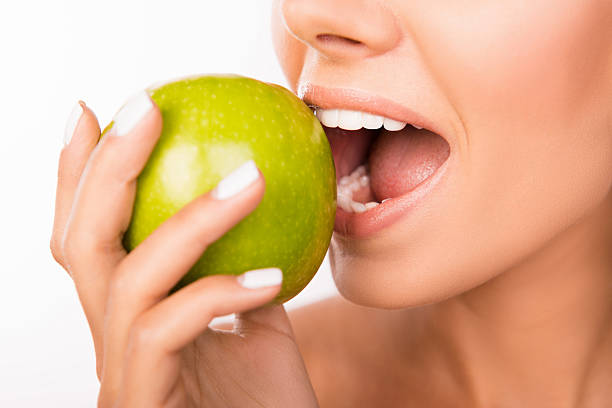
\includegraphics[width=\linewidth]{istockphoto-622282400-612x612.jpg}
\end{tikzfigure}
}

\end{document}